%HEADER

%<---!!!!!!!!!!!!!!! MAKRO-DEFIONITIONEN; BITTE NICHT VERAENDERN !!!!!!!!!!
%<--- ARBEIT EINSEITIG
\def\makroEinseitig{
%KOMA-Script-Klasse: scrreprt
%deutsches Design, Schriftgröße 12, DIN A4
%Literaturverzeichnis und Index in Inhaltsverzerzeichnis einbinden
\documentclass[12pt,a4paper,listof=totoc,oneside]{scrreprt}
%Seitenspiegel einstellen
\usepackage[a4paper]{geometry}
\geometry{a4paper,left=30mm,right=25mm,
bottom=20mm,top=15mm,bindingoffset=2mm,
includehead,includefoot}}
% ARBEIT EINSEITIG --->

\def\makroZweiseitig{
%<--- ARBEIT ZWEISEITIG
%KOMA-Script-Klasse: scrreprt
%deutsches Design, zweiseitig
%Literaturverzeichnis und Index in Inhaltsverzerzeichnis einbinden
\documentclass[12pt,a4paper,listof=totoc,twoside, headsepline]{scrreprt}
\usepackage[a4paper]{geometry}
\geometry{a4paper,left=25mm,right=25mm,
bottom=20mm,top=15mm,bindingoffset=2mm,
includehead,includefoot}}
% ARBEIT ZWEISEITIG --->

%<--- Einstellungen Kopfzeile
\def\makroFH-Kopfzeilenstil{
\pagestyle{scrheadings} 
\setheadsepline{0.4pt}
\pagestyle{scrheadings}
\renewcommand*{\chapterpagestyle}{scrheadings}}
%Einstellungen Kopfzeile --->
%!!!!!!!!!!!!!!! MAKRO-DEFIONITIONEN; BITTE NICHT VERAENDERN !!!!!!!!!!--->


%AUSWAHL: TEXT EINSEITIG (ja/nein)
\makroEinseitig
%\makroZweiseitig

%schalte Umlaute frei
\usepackage[english, ngerman]{babel}
%passende Codierung
\usepackage[utf8]{inputenc}
%Seitenspiegel einzustellen
\usepackage[a4paper]{geometry}

%%%%%%%%%%%%%%%%%%%%%%%%%%%%%%%%%%%%%%%%%%%%%%%%%%%%%%%%%%%%%%%%%%%%%%%%%%%%%%%%
% Deutsche und englische Referenzen
\usepackage{babelbib}

% Utopia Schriftart
\usepackage{utopia}

% Farbige Überschriften
% https://www.overleaf.com/learn/latex/Using_colours_in_LaTeX
\usepackage[dvipsnames]{xcolor}
\usepackage{sectsty}
\chapterfont{\color{CornflowerBlue}}
\sectionfont{\color{Cerulean}}
\subsectionfont{\color{Cerulean}}
\subsubsectionfont{\color{Cerulean}}
\paragraphfont{\color{Cerulean}}
%%%%%%%%%%%%%%%%%%%%%%%%%%%%%%%%%%%%%%%%%%%%%%%%%%%%%%%%%%%%%%%%%%%%%%%%%%%%%%%%

%Mathepaket
\usepackage{amsmath}
%Symbole
\usepackage{amssymb}
%griechische Symbole
\usepackage{upgreek}
%weitere Symbole
\usepackage{pxfonts}
% Phonetischen Alphabete für LaTeX
\usepackage{tipa}
%farbige Schriften
%\usepackage{color}
\usepackage{scrhack}
%Bilder fixieren
\usepackage{float}
%Grafiken einbinden
\usepackage{graphicx}
% Kopf- und Fußzeilen
\usepackage[automark,standardstyle,markusedcase]{scrlayer-scrpage}
% deutsche Überschriften
\usepackage[ngerman]{translator}
% Kopfzeilenabstand festlegen
\setlength{\headheight}{10mm}
%Abb. statt Abbildung
\usepackage{caption3}
\addto\captionsngerman{
\renewcommand{\figurename}{Abb.}
\renewcommand{\tablename}{Tab.}
}
%Glossar-Pakage
% HYPERREF VOR GLOSSARIES EINFÜGEN
\usepackage{hyperref}

\usepackage[
nonumberlist, %keine Seitenzahlen anzeigen
acronym,      %ein Abkürzungsverzeichnis erstellen
toc]          %Einträge im Inhaltsverzeichnis      
{glossaries}
\usepackage{cite}
% degree sign
\usepackage{gensymb}

\hypersetup{ colorlinks,
linkcolor=MidnightBlue,
filecolor=MidnightBlue,
urlcolor=MidnightBlue,
citecolor=MidnightBlue }

%Glossar einschalten
\makeglossaries


%fertigen Kopfzeilenstil aktivieren
\makroFH-Kopfzeilenstil

%Zeilenabstand * 1.25 (default)
\renewcommand{\baselinestretch}{1.25}\normalsize
%(Kommentar entfernen, um Zeilenabstand
% auf 1,5-fache Groesse zu ueberschreiben)
%\renewcommand{\baselinestretch}{1.50}\normalsize

% KOMPILATION
% pdflatex Arbeit_Main.tex
% makeglossaries Arbeit_Main
% bibtex Arbeit_Main
% 2 * pdflatex Arbeit_Main.tex
%

% https://www.overleaf.com/learn/latex/Tables
%\setlength{\arrayrulewidth}{0.5mm}
\setlength{\tabcolsep}{18pt}
\renewcommand{\arraystretch}{1.5}

\newcommand{\todo}[1]{\textcolor{red}{\textbf{TODO #1}}}
\newcommand{\xcom}{\textcolor{YellowGreen}{\textbf{[?] }}}
\newcommand{\misobj}[1]{\textcolor{YellowGreen}{\textbf{#1}}}

\begin{document}

%Befehle für Symbole
%\newglossaryentry{symb:Pi}{
%name=$\pi$,
%description={Die Kreiszahl.},
%}
%\newglossaryentry{symb:Phi}{
%name=$\varphi$,
%description={Ein beliebiger Winkel.}
%}
%\newglossaryentry{symb:Lambda}{
%name=$\lambda$,
%description={Eine beliebige Zahl, mit der der nachfolgende Ausdruck
%multipliziert wird.}
%}

%Akronyme
\newacronym{MS}{MS}{Microsoft}
%\newacronym{CD}{CD}{Compact Disc}
%Eine Akronym mit Glossareintrag
%\newacronym{AD}{AD}{Active Directory\protect\glsadd{glos:AD}}

%Glossareinträge
%\newglossaryentry{glos:AD}{
%name=Active Directory,
%description={Active Directory ist in einem Windows 2000/" "Windows
%Server 2003-Netzwerk der Verzeichnisdienst, der die zentrale ...
%}
%}
\newglossaryentry{glos:AntwD}{name=Antwortdatei, description={Informationen zum
Installieren einer Anwendung oder des Betriebssystems.}}




%Titelseite
% Seitennummer aus
\thispagestyle{empty}
\begin{titlepage}
	\vspace{3cm}

%%\begin{center}
%%	\Huge	
%%	HOCHSCHULE LANDSHUT \\
%%	\Large
%%	FAKULTÄT INFORMATIK
%%\end{center}

%%\vspace{1cm}

\begin{center}
	\includegraphics[scale=0.8]{Grafiken/hl-logo.pdf}  
\end{center}

\vspace{2.5cm}

\begin{center}
  \Large FAKULTÄT INFORMATIK
\end{center}

\vspace{1cm}
\begin{center}
	\Huge
	\textbf{Masterarbeit}\\
\end{center}

\vspace{1cm}

\begin{center}
	\Large
	\textsc{Predictive Analytics im öffentlichen Sektor - Anwendungsmöglichkeiten,
    Chancen und Risiken}\\
\end{center}

\vspace{1.5cm}

\begin{center}
	\Large
	Dmitrij Novikov
\end{center}

\vspace{2cm}
\begin{center}
	\large
	%\the\month\,/\,\the\year
  \today
\end{center}

\vspace{2cm}
\begin{center}
	\large
	Betreuer: Prof. Dr. Wunderlich
\end{center}

\end{titlepage}


%Füge leere Seite ein (optional)
\input{Inhalt/LeereSeite}
%Verwende Muster-Erklärung zur selbstständigen Arbeit 
\input{Inhalt/Erklaerung}
%Füge leere Seite ein (optional)
\input{Inhalt/LeereSeite}

\begin{abstract}
\begin{center}
\Huge
\emph{\textbf{Übersicht}}
\end{center}
\normalsize
\vspace{15mm}
\textit{Forecasting und Predictive Analytics sind zwei evidenzbasierte Methoden,
die helfen können, bessere Urteile zu fällen und bessere Entscheidungen zu
treffen. Allerdings wird die Verbreitung dieser Methoden auf taktischer und
strategischer Ebene schwierig werden, da insbesondere dort Widerstände zu
erwarten sind. Es bleibt zu hoffen, dass der Wille, bessere 
Entscheidungsgrundlagen zu erhalten, stärker ist. Eine Literaturrecherche 
zu der Verbreitung von Predictive Analytics im öffentlichen Sektor ergab, dass
solche Anwendungen hauptsächlich auf operativer Ebene implementiert werden und
bestätigte damit obigen Verdacht.}
\end{abstract}


\tableofcontents
\setcounter{page}{1}

\chapter{Einleitung}
\label{part:Einleitung}

In dieser Arbeit soll die Anwendung von Datenanalysen und insbesondere
von \emph{\gls{glos:Predictive_Analytics}} im öffentlichen Sektor untersucht
werden.
Der Schwerpunkt liegt dabei auf Deutschland, wobei aber auch relevante
Anwendungsgebiete in anderen Staaten betrachtet werden. \\ \\
Der einleitende Teil~\ref{part:Schw_Vorhersagen} soll zunächst das Problem der
Schwierigkeit von
Prognosen untersuchen und damit eine Motivation für die Anwendung von 
\emph{predictive analytics} liefern. \\ \\
In Teil~\ref{part:Konzepte_PA} werden die wichtigsten Konzepte von
\emph{predictive analytics} vorgestellt. Dabei werden auch die allgemeinen
Risiken bei der Anwendung diskutiert. \\ \\
\misobj{weitere Teile}

\chapter{Die Schwierigkeit von Vorhersagen}
\label{part:Schw_Vorhersagen}

Mit Hilfe von \emph{\gls{glos:Predictive_Analytics}} werden Datenanalysen
erstellt, die die Vorhersage von Entwicklungen oder die Einschätzung von
Situationen unterstützen sollen. Dabei werden in der Regel Computeralgorithmen
mit Daten trainiert, um für spätere Abfragen zuverlässige Prognosen zu liefern.
Entscheidungsträgern soll \emph{predictive analytics} also helfen, bessere
strategische Entscheidungen zu treffen (vgl. \cite{Mauerer}, S.~2). %\\ \\
Dies könnte
\begin{description}
\item[(a)] notwendiger sein als erwartet und
\item[(b)] schwieriger werden als gedacht.
\end{description}
Denn eine ausführliche Studie des Psychologen Philip Tetlock aus dem Jahr 2005
(siehe \cite{Tetlock}) ergab,
dass Experten zu politischen Fragen keine besseren Prognosen liefern konnten,
als die einfachsten statistischen Algorithmen. Zudem hatten die Experten
große Schwierigkeiten damit, ihre Prognosen angesichts schlechter Resultate
anzupassen und zu verbessern. \\ \\
Die Experten sollten ihr Können bei mehreren Prognoseaufgaben
(\emph{forecasting exercises}) unter Beweis stellen. Dabei wurden verschiedene
mögliche politische oder wirtschaftliche Ereignisse skizziert und die Experten
sollten subjektiv abschätzen, für wie wahrscheinlich sie es halten, dass das
Ereignis eintritt\footnote{Es sollten numerische Werte angegeben werden. Also
0 für \glqq{Es} ist unmöglich, dass das Ereignis eintritt\grqq und 1 für
\glqq{Das} Ereignis wird mit Sicherheit eintreten\grqq. Werte zwischen 0 und 1
drücken dann einen Grad von Unsicherheit über das Ereignis aus.}.
Nachdem das festgelegte Zeitfenster für die Ereignisse abgelaufen war, konnte
das Eintreten oder Nichteintreten der jeweiligen Szenarien beobachtet werden und
rückblickend mit den Vorhersagen der Teilnehmer abgeglichen werden.  
Zur Messung der Genauigkeit der Vorhersagen wurde eine Maßzahl,
der \emph{probability score} verwendet. Dadurch konnten die Vorhersagen der
menschlichen Teilnehmer mit den Ergebnissen von einfachen und erweiterten
statistischen Algorithmen verglichen werden. \\ \\
Das Ergebnis ist in Abbildung~\ref{pic:Tetlock_1} dargestellt und wird im
folgenden Text ausführlich erläutert\footnote{Die Grafik ist eine leicht 
abgewandelte Version vom Original aus \cite{Tetlock}, S. 51).}. \\ \\
\begin{figure}%[!hbt]
\centering
\caption{Bei den \emph{forecasting exercises} erzielte Wertungen.}
\includegraphics[scale=1.0]{Grafiken/Tetlock_1_Fertig_Ink.pdf} 
\label{pic:Tetlock_1}
\end{figure}
Die zwei
Bestandteile des \emph{probability score}, Kalibrierung (\emph{calibration}) und
Diskriminierung (\emph{discrimination}), sind auf den Achsen abgebildet. \\ \\ 
Kalibrierung (horizontale Achse) misst die Fähigkeit eines Prognostikers,
Ereignisse korrekt nach ihrer
Auftrittswahrscheinlichkeit zu ordnen (vgl. \cite{Tetlock}, S.~47). So ist ein
Prognostiker gut kalibriert, wenn etwa 10~\% der Ereignisse eintreten, für die
er eine Wahrscheinlichkeit von 0.1 geschätzt hat, 20~\% der Ereignisse eintreten
die eine Wahrscheinlichkeit von 0.2 erhalten haben, und so weiter. Je kleiner
der numerische Wert der Kalibrierung, desto besser ist der Prognostiker. Bei
einem Wert von 0 ist die bestmögliche Kalibrierung erreicht und aus diesem Grund
ist (1 - Kalibrierung) auf der horizontalen Achse abgebildet. \\ \\
Weiterhin ist ein Prognostiker umso besser bei der Diskriminierungskomponente
(vertikale Achse),
je eher es ihm gelingt die Auftrittswahrscheinlichkeiten von einzelnen
Ereignissen von der relativen Häufigkeit aller Ereignisse\footnote{
genauer: Das Verhältnis der Anzahl der eingetretenen Ereignisse zu der
Gesamtanzahl der Ereignisse} (\emph{base-rate})
zu unterscheiden. Perfekte Diskriminierung wird erreicht, wenn allen 
eingetretenen Ereignissen eine Wahrscheinlichkeit von 1.0 zugeordnet wird, und
alle Ereignisse, die nicht eingetreten sind, mit Null bewertet werden
(vgl. \cite{Tetlock}, S.~47).\\ \\
Nun gehen Kalibrierung und Diskriminierung als Summe in den
\emph{probability score} ein. Aus diesem Grund kann sich für verschiedene
Werte von Kalibrierung und Diskriminierung der gleiche Wert für den
\emph{probability score} ergeben. Die diagonalen Linien in Abbildung~\xcom
markieren Stellen mit konstantem \emph{probability score}. Je weiter rechts oben
eine Linie verläuft, desto höher ist der zugehörige \emph{probability score}.
\\ \\
Die Gesamtergebnisse für Kalibrierung und Diskriminierung für die verschiedenen
Teilnehmergruppen sind in der Graphik eingetragen. Die am besten qualifizierte
Gruppe stellen die Experten dar, die Fragen zu ihren jeweiligen Fachgebieten
erhalten haben (vgl. \cite{Tetlock}, S.~242). Weniger qualifiziert sind die 
\glqq{Dilettanten}\grqq (\emph{dilettantes}), Experten, die jedoch Fragen
beantwortet haben, die nicht zu ihrem Spezialgebiet gehören. Die Dilettanten
gaben an, dass sie sich mit Hilfe qualititativ hochwertiger Quellen
(\emph{Economist}, \emph{Wall Street Journal}, \emph{New York Times} etc.) über
Themen außerhalb ihrer Fachgebiete informieren (vgl. \cite{Tetlock}, S.~56).
Die Gruppe mit der geringsten Qualifikation waren Studenten, die die Übungen
zu Vorhersagen absolvieren mussten, nachdem sie kurze Zusammenfassungen von
Fakten zu den jeweiligen Themen erhalten haben (vgl. \cite{Tetlock}, S.~56).
\\ \\
Weiterhin enthält Abbildung~\ref{pic:Tetlock_1} auch die Ergebnisse, die von den
statistischen Algorithmen erzielt wurden. Zur besseren Übersicht werden die
Algorithmen hier in vier Gruppen eingeteilt. Der Stufe 0 Algorithmus würfelt
einfach die Antworten , er ordnet den zur Debatte stehenden Ereignissen
zufällige Wahrscheinlichkeiten zu. Weiterhin gibt es mehrere Varianten von
Stufe 1 Algorithmen, die als Antwort auf die Fragen immer die relative
Häufigkeit der Ereignisse eintragen. Etwas komplexer sind die Stufe 2
Algorithmen. Diese extrapolieren aus der Vergangenheit in die Zukunft und setzen
die Wahrscheinlichkeiten für die Ereignisse entsprechend. Die höchste
Komplexität hat der Stufe 3 Algorithmus. Um die Eintrittswahrscheinlichkeiten
der Ereignisse zu ermitteln, nutzt dieser die Vergangenheitswerte mehrerer
Variablen, die eine hohe Vorhersagekraft besitzen.\footnote{Die genaue Zuordnung
der Stufen 0-3 zu den Algorithmen in der Originalquelle (\cite{Tetlock}, S.~51)
sieht folgendermaßen aus:
\begin{description}
\item[Stufe 0:] \emph{random guessing} (\emph{chimp})
\item[Stufe 1:] \emph{contemporary base rate} (1-1), \emph{restrictive base
  rate} (1-2), \emph{expansive base rate} (1-3)
\item[Stufe 2:] \emph{cautious case-specific extrapolation} (2-1),
  \emph{aggressive case-specific extrapolation} (2-2)
\item[Stufe 3:] \emph{autoregressive distributed lag models}
\end{description}
} \\ \\
Abbildung~\ref{pic:Tetlock_1} zeigt, dass die Experten die Studenten bei
den \emph{forecasting exercises} deutlich schlagen konnten. Allerdings waren die
Experten kaum besser (!) als der zufallsgesteuerte Algorithmus 
(Stufe 0)\footnote{Die Experten waren schlechter kalibriert aber besser bei
der Diskriminierung, sodass sie insgesamt eine etwas bessere Gesamtwertung
hatten}. Insbesondere verloren die Experten gegen die komplexeren Algorithmen
(Stufe 2 und 3) mit deutlichem Abstand und zwar sowohl bei Kalibrierung, als
auch bei Diskriminierung. Falsche Überzeugungen und mentale Barrieren haben, so
Tetlock, das Urteilsvermögen der Experten getrübt und zu den schlechten
Ergebnissen geführt (mehr dazu in Abschnitt~\xcom). \\ \\
Was haben diese Ergebnisse mit \emph{predictive analytics} und dem öffentlichen
Sektor zu tun?\\ \\
Erstens waren die Fragestellungen der \emph{forecasting exercises} aus den
Bereichen Politik und Wirtschaft\footnote{
Andere Themen, wie beispielweise naturwissenschaftliche Fragestellungen,
z. B. \glqq{Wie} wahrscheinlich ist die Detektion dunkler Materie
in den nächsten fünf Jahren?\grqq, wurden nicht behandelt.
}, was für den öffentlichen Sektor relevant ist. Zweitens handelt es sich dabei
um generelle Probleme der menschlichen Urteilsfindung. Probleme, die in vielen
Bereichen auftreten und zu Fehleinschätzungen führen können. Zudem
konnten datenbasierte Algorithmen, also \emph{predictive analytics}, die
menschlichen Vorhersagen bei den \emph{forecasting exercises} schlagen. Dies
deutet darauf hin, dass formale Methoden wie \emph{predictive analytics} dabei
helfen können, bessere Urteile zu fällen und folglich auch bessere
Entscheidungen zu treffen. \\ \\
Der nächste Teil der Arbeit behandelt \emph{predictive analytics},
den Prozess der (menschlichen) Urteilsfindung und wie formale Methoden diesen
Prozess verbessern können.


\chapter{Konzepte von Predictive Analytics}
\label{part:Konzepte_PA}

\section{Begriffsdefinition und -Abgrenzung}

\section{Bestandteile von Predictive Analytics}

\subsection{CRISP-DM Vorgehensmodell}

\subsection{Daten}

\subsubsection{Information Management (Data Warehouse)}

\subsubsection{Datenabhängige Ziele}

\paragraph{\ldots}

\paragraph{Beschreibung der Daten}

\paragraph{Klassifikation}

\paragraph{Zeitreihenanalyse}

\subsection{Methoden}

\subsubsection{Die Großen Drei}

\paragraph{Regression}

\paragraph{Entscheidungsbäume}

\paragraph{Neuronale Netze}

\subsubsection{Zeitreihenanalyse}

\subsubsection{\ldots}

\subsection{Werkzeuge}

\subsection{(Kreative) Freiheitsgrade bei der Implementierung eines
  Vorhersagemodells}

\section{Anwendungsbeispiele}

\subsection{Allgemeine Anwendungsfelder (siehe SAP Artikel)}

\subsection{\ldots}

\section{Allgemeine Risiken bei der Nutzung von Predictive Analytics}

Es exisitieren Risiken, die dazu führen können, dass die Ziele einer
Datenanalyse nicht oder nicht in vollem Umfang erreicht werden können.
Im folgenden Text werden einige dieser Risiken erläutert.

\subsection{Risiko der Unverhältnismäßigkeit}

Die Anwendung von Predictive Analytics ist mit einem hohen Aufwand verbunden.
Dabei spielen die Kosten für die Datenerhebung eine wesentliche Rolle.
Zusätzlich werden für die Datenanalyse Kenntnisse aus verschiedenen
Fachrichtungen benötigt. So sind einerseits anwendungsspezifische Kenntnisse
zur Interpretation der Daten und der Ergebnisse wünschenswert. Andererseits
werden zur Durchführung der Datenanalyse Kenntnisse in Mathematik, Statistik und
Informatik benötigt. \\ \\
Aus diesem Grund besteht das Risiko, dass die Kosten einer Anwendung von
Predictive Analytics den Nutzen übersteigen. Es ist auch möglich, dass das
gleiche Ergebnis mit einer einfacheren, kostengünstigeren Methode erreicht
werden kann. In diesem Fall würde die Anwendung eines aufwändigen Predictive
Analytics Verfahrens wertvolle Ressourcen binden, die an anderer Stelle stärker
gebraucht werden. \\ \\
Somit ist es wichtig, Betrachtungen zu Alternativkosten \todo{gls eintrag}
in die 
Planung von Predictive Analytics Anwendungen einzubeziehen. 

\subsection{Risiken bei der Datenerhebung}

\subsubsection{\ldots}

\subsection{Risiken bei der Interpretation der Daten}

\subsection{Risiken bei der Interpretation der Ergebnisse}

Wenn die Ergebnisse der Datenanalyse zur Entscheidungsunterstützung herangezogen
werden, beeinflussen sie das Verhalten der Entscheidungsträger. Dies kann zur
Entstehung problematischer psychosozialer Effekte führen. Zwei Beispiele hierfür
werden nun erläutert.

\subsubsection{Prognose verändert das Verhalten des Systems 
%  (``Selffulfilling Prophecy'')}
  (\glqq{Selffulfilling} Prophecy\grqq)}

\subsubsection{Ignorieren der Unsicherheiten bei der Prognose}

Es besteht die Gefahr, dass die Unsicherheiten von Vorhersagen ignoriert werden
und die Prognose als eine Gewissheit betrachtet wird. Somit wird möglichen,
alternativen Entwicklungen bei der Entscheidungsfindung nicht genügend Bedeutung
beigemessen. Dies kann dazu führen, dass Risiken falsch kalkuliert werden und
in der Zukunft nicht genügend Handlungsoptionen zur Verfügung stehen.


\chapter{Predictive Analytics im öffentlichen Sektor}

% TODO
% Stand Entscheidungshilfen (wie vorstellbar: Mensch entscheidet, Computer
%   unterstützt)
% Abgrenzung zum privaten Sektor
% auf operativer Ebene allerdings ähnlich

% s. Watson, Abschnitt Lack of regulation and algorithm bias
% TODO bias insgesamt (in Rahmenbedingungen)
\begin{figure}%[!hbt]
\centering
\caption{Risikomatrix für die Nutzung maschineller Entscheidungshilfen}
\includegraphics[scale=1.0]{Grafiken/Risk_Matrix_Ink.pdf} 
\label{pic:Risiko_Matrix}
\end{figure}

\section{Rahmenbedingungen}

% TODO
% Rahmenbedingungen:
% - Wahrheit taktisch genutzt
% - versch. Gruppen/Kulturen -> versch. Wahrheiten
% - Themen kontroverser (vs. z. B. Fruchtsäfte)
% - Konkurrenz (v. a. bei strategischen Entscheidungen) 
% - Ignorieren (-> Probleme menschl. Urteile)

\section{Spieltheoretische Betrachtung}

% TODO


% deadlock (S. 218(
\begin{figure}%[!hbt]
\centering
\caption{Deadlock Auszahlungsmatrix}
\includegraphics[scale=0.8]{Grafiken/Deadlock_Ink.pdf} 
\label{pic:Deadlock}
\end{figure}

% stag hunt (S. 220)
\begin{figure}%[!hbt]
\centering
\caption{Stag Hunt Auszahlungsmatrix}
\includegraphics[scale=0.8]{Grafiken/Stag_Hunt_Ink.pdf} 
\label{pic:StagHunt}
\end{figure}

% mixed
\begin{figure}%[!hbt]
\centering
\caption{Gemischte Stag Hunt-Deadlock Auszahlungsmatrix}
\includegraphics[scale=0.8]{Grafiken/Mixed_Ink.pdf} 
\label{pic:Mixed}
\end{figure}

% prisoners dilemma (S.237)
% mixed
\begin{figure}%[!hbt]
\centering
\caption{Gefangenendilemma Auszahlungsmatrix}
\includegraphics[scale=0.8]{Grafiken/Prisoner_Ink.pdf} 
\label{pic:Prisoner}
\end{figure}
%-------------------------------------------------------------------------------
\section{Anwendungen von Predictive Analytics im öffentlichen Sektor}

% Auswahl
% TODO Fallstudien einfach ausführlichere Beispiele

\subsection{Öffentliche Verwaltung}

% TODO
% Daten in der öffentlichen Verwaltung
% Open Data Portale ( GovData.de )
% Abgrenzung zu 'Nowcasting'
% Predictive Analytics in Finanzbehörden
% Predictive Policing
% Einschätzung der politischen Stimmungslage
% Vorhersage kultureller Unterschiede

\subsubsection{Cambridge Analytica - Fallstudie}

\begin{figure}%[!hbt]
\centering
\caption{Nutzung von Facebook Likes zur Vorhersage von Nutzerattributen}
\includegraphics[scale=1.0]{Grafiken/Facebook_Likes_Ink.pdf} 
\label{pic:Like_Matrix}
\end{figure}

\subsection{Öffentliche Gesundheit}

% TODO
% Google Flu Trends (vorerst gescheitert)
% Kohortenstudien nützlich bei: bsp. Kampagnen zur öffentlichen Gesundheit
%   bsp. Ernährungskampagnen, Anti-Rauch-Kampagnen 
% Kohortenstudien: nicht persönlich (s. Watson, Abschnitt Cohort treatment),
%   aber Sicherheitsbedenken bleiben (Anonymisierung nicht möglich, Sicherheits
%   risiken ...)
\subsubsection{Flint Trinkwasserskandal - Fallstudie}

\subsection{Bildung}

% Anwendungsbeispiel Decision Tree

% TODO echten Titel ersinnen
\chapter{Zusammenfassung und Fazit}

%%%%%%%%%%%%%%%%%%%%%%%%%%%%%%%%%%%%%%%%%%%%%%%%%%%%%%%%%%%%%%%%%%%%%%%%%%%%%%%%
\appendix
% TODO evtl umbennen 
\chapter{Probablility Scoring - Vertiefung}

% TODO
% Brier Score Erklärung
% Brier Score Probleme
%   Vorhersage unwahrscheinlicher Ereignisse nicht gewürdigt
%   50/50 fence sitters -> unbefriedigend, Frustration (need for closure)
%   % S. 276 Indiscriminate fence-sitting
% Bayes Belief Updating Erklärung/Herleitung
% Kognitive Verzerrungen, Auflistung, Diskussion
%   Erlernbar oder nicht (- individuell nicht gelungen, + in Gruppe, 
%     Kommunikation hilft, Unterschiede nicht unüberwindbar)
% + eher statistisch, mathematische "Verzerrungen" (subadditivity ...)
% 11 Commandments GJP

\chapter{Predictive Analytics mit R}

% TODO
% Kurzvorstellung R, Vergleich mit anderen Werkzeugen (insb. Python)
% vllt R stark in Grafik
% R Verwendung in Verwaltungen

%%%%%%%%%%%%%%%%%%%%%%%%%%%%%%%%%%%%%%%%%%%%%%%%%%%%%%%%%%%%%%%%%%%%%%%%%%%%%%%%
% TODO vllt Zusatzmaterial:

% Tetlock S. 63: systematic distortions in the media markets for intellectual
%   commentary

% Bayes belief updating konvergiert (Arens)



%%%%%%%%%%%%%%%%%%%%%%%%%%%%%%%%%%%%%%%%%%%%%%%%%%%%%%%%%%%%%%%%%%%%%%%%%%%%%%%%
\listoffigures
\listoftables
\printglossary[title=Glossar]
\printglossary[type=\acronymtype, title=Akronyme]
% keine deutschen Überschriften
%\printglossaries 

\bibliography{Bibliographie/Bibli.bib}{}
\bibliographystyle{babplain}

\end{document}


